\section{Experiments}

In this section, we provide the experimental results on design choices for different parts of the model. The majority of experiments are done on the cluster, and finally, we transfer the model to a mobile device to check the performance there.

\subsection{Implementation details}

The models were implemented in PyTorch using Detectron2 \cite{detectron2} platform.

We choose hyper-parameters matching to those in Parsing R-CNN\cite{parsing}, i.e., we use a batch of 16 images (2 images per GPU), therefore we apply synchronous batch normalization \cite{syncbn} instead of usual batch normalization wherever it is used inside the backbone and neck. We use no normalization in box/class and dense pose heads. We sample 512 RoIs for box/class head and 32 RoIs for dense pose head. By default, we train models for 130k iterations with initial learning rate 0.002, decreasing it by 10 at 100k and 120k iterations. Under such a schedule, training of one model takes approximately 1 day on 8 NVIDIA Tesla V100 GPUs. Since all models are quite small, the memory consumption during training allows to decrease the number of GPUs for parallel training. Unless specified otherwise, by default, we scale images in a way that shortest image size equals 800 pixels during the inference stage. Each model's backbone is initialized with weights of the corresponding network trained on the ImageNet classification task. We train models on a combination of \textit{train} and \textit{valminusminival} partitions of Densepose-COCO dataset \cite{densepose} and test them on a \textit{minival} partition.


\subsection{Metrics}
Following the original work, we use as evaluation metric the Average Precision (AP) at a number of \textit{geodesic point similarity} (GPS) thresholds ranging from 0.5 to 0.95. We also report box average precision.

As we are interested in deploying a DensePose model on a mobile device, we report the number of parameters of each model and FPS measured on CPU and GPU. In particular, we measure the inference performance of all models on the same NVIDIA GeForce GTX 1080 Ti. It is worth mentioning that the DensePose model is a two-stage model, so the FPS of the model is directly conditioned on the performance of the first stage of the model. There is a subtle trade-off between the quality and latency; as for example, the network that does not predict any instances will never run dense pose head, and vice versa, the network that produces many false-positive results would redundantly run the model heads. As the latency of the network is data-dependent, we average latency time across DensePose-COCO minival dataset and finally convert it to FPS.

\subsection{Ablation on components}

\begin{table*}[t!]
\centering
\resizebox{\textwidth}{!}{
\begin{tabular}{cllll}
 &  DensePose R-CNN (baseline) \cite{densepose} & Parsing R-CNN \cite{parsing} & Mobile Parsing R-CNN (A) & Mobile Parsing R-CNN (B) \\\hline
Backbone & ResNet-50 \cite{resnet} & ResNet-50 \cite{resnet} & Single-Path \cite{spnasnet} & Single-Path \cite{spnasnet} \\
Neck & FPN\cite{fpn} & FPN\cite{fpn} & FPN\cite{fpn} & BiFPN  \\
RoI resolution & $14\times14$ & $32\times32$ & $32\times32$ & $32\times32$ \\
Pooling Type & RoIPool & RoIPool & RoIAlign & RoIAlign \\
Box/class head & 2 linear layers & 2 linear layers & 2 conv layers & 2 conv layers \\
% test time shortest image size & 800px & 800px & 800px & 800 px\\
Feature level for prediction & $P_2$,$P_3$,$P_4$,$P_5$ & $P_2$ & $P_2$ & $P_2$ \\
DensePose head & 8 conv layers & ASPP\cite{aspp}+NL\cite{nonlocal}+4 conv layers & ASPP\cite{aspp}+4 conv layers & ASPP\cite{aspp}+4 conv layers \\
\#Channels & 512 & 512 & 256 & 64 \\
\hline
\#Params & 59.73M & 54.36M & 11.35M & 3.35M \\
GPU FPS & $13.16$ & $10.15$ & $12.03$ & $22.77$ (3x LR: $\mathbf{23.55}$) \\
CPU FPS & $1.62$ & $1.39$ & $1.42$ & $2.02$  (3x LR: $\mathbf{2.10}$) \\
box AP & $57.8$ & $59.609$ & $56.370$ & $55.39$ (3x LR: $56.83$)\\
densepose AP & $49.8$ & $54.676$ & $49.512$ & $46.79$ (3x LR: $51.08$)\\
\hline
\end{tabular}}
\caption{The main differences between the models presented. Results on DensePose-COCO minival. 3x LR refers to 3 times longer training compared to the default setting. $P_i$ represents a feature level with a resolution of $1/2^i$ of the input images. \#Channels represent the number channels inside \textit{neck} and \textit{heads}.}
\label{table:configs}
\end{table*}

% TODO describe testing pipeline

% In this section we show how we accelerated Parsing R-CNN architecture for dense pose estimation task.

% TODO highlight the differences 
\begin{table*}[t!]
\centering
\resizebox{\textwidth}{!}{
\begin{tabular}{lcccccc}
\hline
Backbone & Top-1 Accuracy (\%) & \#Params & box AP & dp. AP & GPU FPS & CPU FPS \\ \hline
ResNet-50 \cite{resnet} & $77.15$ & $33.61$M & $60.0$ & $\mathbf{54.7}$ & $11.05$ & $1.34$ \\
EfficientNet-B3 \cite{efficientnetb} & $81.636$ & $16.03$M & $59.027$ & $53.084$ & $8.31$ & $1.37$ \\
EfficientNet-EdgeTPU-L \cite{efficientnete} & $80.534$ & $17.89$M & $60.069$ & $53.378$ & $8.11$  & $1.34$ \\
MixNet-XL \cite{mixnet} & $80.120$ & $19.10$M & $58.444$ & $51.475$ & $8.54$  & $1.32$ \\
EfficientNet-B2 \cite{efficientnetb} & $79.688$ & $13.68$M & $58.041$ & $51.800$ & $9.33$ & $1.38$ \\
MixNet-L \cite{mixnet} & $78.976$ & $14.62$M & $57.481$ & $50.649$ & $8.52$ & $1.34$ \\
EfficientNet-EdgeTPU-M \cite{efficientnete} & $78.742$ & $14.57$M & $58.825$ & $52.302$ & $9.21$ & $1.37$ \\
EfficientNet-B1 \cite{efficientnetb} & $78.692$ & $13.03$M & $57.654$ & $51.053$ & $9.49$ & $1.39$ \\
CondConv-EfficientNet-B0 \cite{efficientnete, condconv} & $77.304$ & $18.32$M & $56.779$ & $49.231$ & $10.63$ & $1.40$ \\
EfficientNet-EdgeTPU-S \cite{efficientnete} & $77.264$ & $13.12$M & $58.296$ & $51.606$ & $10.03$ & $1.39$ \\
MixNet-M \cite{mixnet} & $77.256$ & $12.39$M & $56.834$ & $48.371$ & $9.39$ & $1.35$ \\
EfficientNet-B0 \cite{efficientnetb} & $76.912$ & $12.10$M & $56.271$ & $49.647$ & $10.53$ & $1.39$ \\
MixNet-S \cite{mixnet} & $75.988$ & $11.52$M & $55.132$ & $46.685$ & $10.34$ & $1.37$ \\
MobileNetV3-Large-1.0 \cite{mobilenetv3} & $75.516$ & $12.04$M & $54.537$ & $47.195$ & $11.54$ & $1.40$ \\
MnasNet-A1 \cite{mixnet} & $75.448$ & $10.94$M & $54.648$ & $47.036$ & $11.21$ & $1.38$ \\
FBNet-C \cite{fbnet} & $75.124$ & $11.49$M & $55.399$ & $47.983$ & $10.97$ & $1.37$ \\
MnasNet-B1 \cite{mnasnet} & $74.658$ & $11.31$M & $52.280$ & $47.658$ & $11.24$ & $1.37$ \\
Single-Path \cite{spnasnet} & $74.084$ & $11.35$M & $56.370$ & $49.512$ & $\mathbf{12.03}$ & $\mathbf{1.42}$ \\
MobileNetV3-Large-0.75 \cite{mobilenetv3} & $73.442$ & $10.92$M & $52.763$ & $44.736$ & $11.02$ & $1.36$ \\
MobileNetV3-Large-1.0 (minimal) \cite{mobilenetv3} & $72.244$ & $10.48$M & $52.464$ & $44.632$ & $11.33$ & $1.36$ \\
MobileNetV3-Small-1.0 \cite{mobilenetv3} & $67.918$ & $10.07$M & $49.614$ & $35.808$ & $10.62$ & $1.35$ \\
MobileNetV3-Small-0.75 \cite{mobilenetv3} & $65.718$ & $9.74$M & $44.224$ & $32.650$ & $10.16$ & $1.33$ \\
MobileNetV3-Small-1.0 (minimal) \cite{mobilenetv3} & $62.898$ & $9.58$M & $45.989$ & $36.522$ & $10.34$ & $1.34$ \\\hline
\end{tabular}}
\caption{Ablation on the backbone network used in Mobile Parsing R-CNN (A). The backbones are sorted by top-1 accuracy. Results on DensePose-COCO \textit{minival}}
\label{table:backbones}
\end{table*}

First, we implemented the Parsing R-CNN \cite{parsing} in Detectron2 following the original implementation. Then we modify the architecture exploiting the techniques presented in the Section~\ref{section3} and present two versions of a new model: Mobile Parsing R-CNN (A) and Mobile Parsing R-CNN (B). See the main architecture differences and obtained results in Table~\ref{table:configs}. Parsing R-CNN outperforms the baseline DensePose R-CNN model by $4.9$ AP, while the Mobile Parsing R-CNN (A) becomes more light-weight with the densepose AP similar to that achieved by the baseline model. The qualitative comparison can be seen in Fig.~\ref{fig:fconfigs}.

Specifically, Mobile Parsing R-CNN (A) is evolved from Parsing R-CNN by careful choice of a backbone, removing non-local block \cite{nonlocal}, decreasing the number of channels in FPN and all heads. Finally, we replace linear layers with convolutional ones in a box/class head. The results of a backbone comparison for Mobile Parsing R-CNN (A) can be seen in Table~\ref{table:backbones}. We use the backbones pretrained on ImageNet from \cite{geffnet}. First, we see that ResNet-50 provides a solid baseline both in terms of AP and FPS. The good FPS can be explained by the fact that the ResNet-50 is one of the first widespread popular deep networks, and GPU manufacturers constantly include this model for bench-marking. In the meantime, other networks contain specific new custom layers and are mainly designed for mobile or embedded devices. Nevertheless, by analyzing results in the Table~\ref{table:backbones}, we pick the Single-Path \cite{spnasnet} backbone as a network providing a good balance between FPS and the dense pose AP.

We move on from Mobile Parsing R-CNN (A) to Mobile Parsing R-CNN (B), by introducing a  new feature aggregation module (BiFPN \cite{bifpn} instead of FPN \cite{fpn}) and further decreasing the number of channels in the dense pose head by a factor of 4, thus 8 times lower than in the baseline architecture. The individual effects of each change can be found in Table~\ref{table:channels}. The transfer from FPN to BiFPN results in a reduced number of parameters,  better box, and densepose AP and the identical FPS. The $4\times$ decrease of the number of channels in BiFPN and all heads results only in $6.0$ densepose AP reduction, while increasing FPS approximately $2$ times.


Our implementation of BiFPN differs from the original one in terms of up-sampling and down-sampling procedure type used to make features from different levels of backbone spatially compatible for the fusion. While the original work uses a bilinear (up)down-sampling, we use a nearest-neighbor variant since we found it to be much faster on mobile devices, and the drop in AP is very slight. Also, in the case of BiFPN, we use features before point-wise linear $1\times1$ convolutions, compared to ``after'' in case of FPN, as it results in slight improvement of dense pose AP. Finally, we train the model three times more iterations, i.e., 390k iterations, reducing learning rate by 10 at 330k and 370k iterations and call it Mobile Parsing R-CNN (B s3x).

\begin{table*}[t!]
\centering
\resizebox{0.8\textwidth}{!}{
\begin{tabular}{cccccccc}
\hline
 & Neck & \#channels & \#Params & box AP & dp. AP & GPU FPS & CPU FPS  \\\hline
Mobile Parsing R-CNN (A) & FPN & $256$ & $11.35$M & $56.371$ & $49.512$ & $12.03$ & $1.42$ \\
 & BiFPN & $256$ & $10.53$M & $58.106$ & $52.80$ & $12.05$ & $1.41$ \\
& BiFPN & $112$ & $4.41$M & $56.41$ & $49.64$ & $19.04$ & $1.78$ \\
& BiFPN & $88$ & $3.82$M & $56.08$ & $48.19$ & $20.43$ & $1.87$ \\
Mobile Parsing R-CNN (B) & BiFPN & $64$ & $3.35$M & $55.39$ & $46.79$ & $22.77$ & $2.02$ \\\hline
\end{tabular}}
\caption{Ablation on neck type and number of channels. The number of channels is the same in neck and heads. Results on DensePose-COCO \textit{minival}}
\label{table:channels}
\end{table*}

% TODO: somehow highlite the differences or move to appendix
\begin{figure*}[t!]
\centering
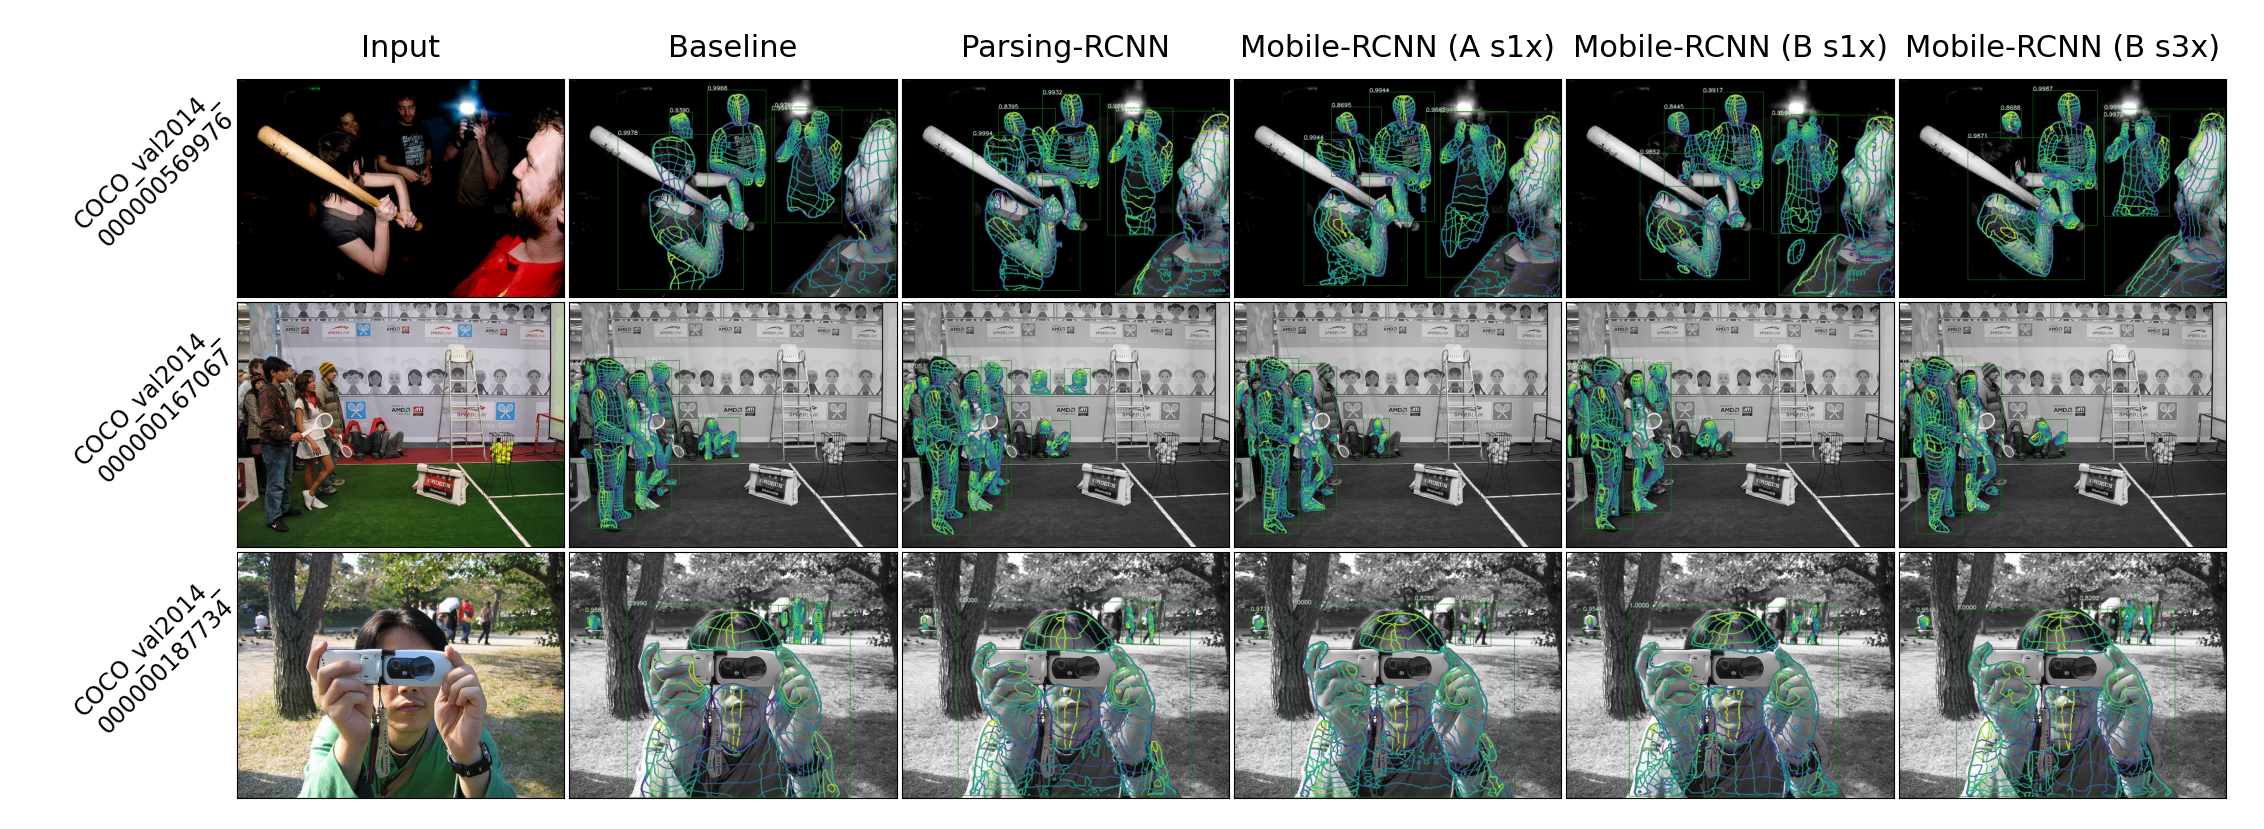
\includegraphics[width=0.9\textwidth]{Figures/densepose/qconfigs_decr.png}
\caption{Qualitative comparison of different models. We depict contours with color-coded U and V coordinates as an output of the model.}
\label{fig:fconfigs}
\end{figure*}

\begin{figure*}[t!]
\centering
\includegraphics[width=0.8\textwidth]{Figures/densepose/mob_comp2.png}
\caption{Qualitative comparison of different backends. We depict contours with color-coded U and V coordinates as an output of the model.}
\label{fig:configs}
\end{figure*}

\subsection{Smartphone-based implementation}


\begin{table*}[t!]
\centering
\resizebox{0.8\textwidth}{!}{
\begin{tabular}{cccccc}
\hline
image shortest side & box AP & dp. AP & GPU FPS & CPU FPS & mobile CPU FPS\\\hline
200px & 36.449 & 19.028 & 27.549 & 10.277 & 2.355\\
400px & 49.181 & 43.916 & 24.648 & 6.921 & 0.954\\
512px & 51.709 & 47.887 & 26.970 & 4.976 & 0.640\\
600px & 53.423 & 49.675 & 25.669 & 4.290 & 0.498\\
800px & 54.744 & 50.560 & 24.033 & 3.046 & N/A\\
1000px & 55.163 & 49.466 & 20.061 & 2.071 & N/A\\\hline
\end{tabular}}
\caption{The impact of image size. Results are obtained with Mobile Parsing R-CNN (B s3x, test-tuned) on DensePose-COCO \textit{minival}. The N/A values correspond to tensor sizes that produced errors on mobile device}
\label{table:pixel}
\end{table*}

\begin{table*}[t!]
\centering
\resizebox{0.9\textwidth}{!}{
\begin{tabular}{ccccccccccc}
\hline
max \# of people & box AP & box APs & box APm & box APl & dp. AP & dp. APm & dp. APl & GPU FPS & CPU FPS & mobile CPU FPS\\\hline
1 & 83.110 & - & 83.389 & 83.173 & 54.329 & 48.203 & 54.765 & 27.508 & 5.859 & 0.684 \\
2 & 74.700 & 24.058 & 56.672 & 77.359 & 52.402 & 47.694 & 52.991 & 27.729 & 5.626 & 0.664 \\
3 & 71.508  & 16.357 & 54.621 & 76.280 & 52.324 & 47.973 & 52.905 & 26.767 & 5.584 & 0.638 \\
4 & 68.818 & 19.532 & 52.693 & 75.693 & 52.050 & 43.131 & 52.838 & 27.198 & 5.510 & 0.606 \\
5 & 66.756 & 20.252 & 53.543 & 74.807 & 51.468 & 44.154 & 52.501 & 27.732 & 5.443 & 0.603 \\\hline
\end{tabular}}
\caption{The impact of number of people in the frame on performance characteristics. Results are obtained with Mobile Parsing R-CNN (B s3x, test-tuned) on DensePose-COCO \textit{minival}. The shortest image side is 512 pixels}
\label{table:people}
\end{table*}

We evaluate the mobile model with Caffe2 runtime, running on a smartphone with ARM processor with 8 cores, 8 threads, and the highest core clock of 2600 MHz.

We use the deployment conversion tools provided by Detectron2 \cite{detectron2}. Specifically, the network is transferred first to ONNX format, then to Caffe2 format.

% \textbf{MODEL.RPN.POST_NMS_TOPK_TEST 100 MODEL.ROI_HEADS.NMS_THRESH_TEST 0.3}
In general, two-stage models introduce numerous hyper-parameters. In case of test-time hyper-parameters, we found empirically, among many different options, that choosing $100$ instead of $1000$ region proposals per \textit{neck} level after non-maximum suppression (NMS) in RPN and changing IoU threshold in NMS from $0.5$ to $0.3$ leads to a significant boost of the model. Therefore later, we use this setup of the model and call it Mobile Parsing R-CNN (B s3x test-tuned).

We check the impact of the image size on the model (see Table~\ref{table:pixel}). The lower resolution of the image, the faster inference we get, but the reduction of image size results in a reduction of densepose AP. In the case of mobile inference, we apply the model on images with the shortest side of size 512 pixels, because it is the lowest resolution processed by the model during the training phase.


% TODO put a number on % of images with less than 5 people 
We are mostly interested in practical applications on the end-device with data fed straight from the device's camera. In this case, usually, the limited number of people appears in the frame. We test the model performance on filtered versions of COCO-DensePose minival partition, where the filtering is based on the maximum number of people in the image. The results can be seen in Table~\ref{table:people}. One can see that the fewer people are in the image, the better performance of the model in AP and FPS. Usually, the fewer people in the image, the more area each person occupies in the frame, which leads to more accurate predictions.

\subsection{Model quantization results}

Here we report the performance statistics of the model obtained using the quantization approach described in Section~\ref{quant}. Thanks to the quantization, we increased the speed of inference by a factor of two and decreased the model size by a factor of three. See exact values in Table~\ref{table:quant}.


\begin{table}[!t]
\centering
\resizebox{0.4\textwidth}{!}{
\begin{tabular}{cccccc}
\hline
weights type & model size & dp. AP & CPU FPS \\\hline
float32 & 13.8mb & 47.887 & 4.976 & \\
int8 & 4.3mb & 44.033 & 8.310 & \\\hline
\end{tabular}}
\caption{The effect of quantization. Results are obtained with Mobile Parsing R-CNN (B s3x, test-tuned) on DensePose-COCO minival. The shortest image side is 512 pixels}
\label{table:quant}
\end{table}